\NeedsTeXFormat{LaTeX2e}

\documentclass[12pt]{article}
\usepackage[letterpaper,portrait, margin=1in, headheight=0.25in]{geometry}
\usepackage{booktabs, pgfplots, bm, multirow, amsmath,fancyhdr}
\pgfplotsset{width=11cm,compat=1.9}
\renewcommand{\arraystretch}{1.5}
\usepackage[colorlinks=true, allcolors=blue]{hyperref}
\usepackage{indentfirst}

\begin{document}
\section{Waves}
\noindent Maxwell Equations:
\begin{equation}
    \nabla\cdot \vec{E}=0
\end{equation}
\begin{equation}
    \nabla\cdot \vec{B}=0
\end{equation}
\begin{equation}
    \nabla\times \vec{E}=-\frac{\partial\vec{B}}{\partial t}
\end{equation}
\begin{equation}
    \nabla\times \vec{B}=\mu_0\epsilon_0\frac{\partial\vec{E}}{\partial t}
\end{equation}
Plane waves propagate in one direction and have uniform $\vec{E}$ fields perpendicular to the direction of propagation.\\
1D Scalar Wave equation:
\[\frac{\partial^2 E_x}{\partial t^2}=\frac{1}{\mu_0\epsilon_0}\frac{\partial^2 E_x}{\partial z^2}\]
3D wave equation:
\[  \nabla^2\psi=\frac{1}{v^2}\frac{\partial^2\psi}{\partial t^2}\]
Wave vector: \[\vec{k}=k_x\hat{x}+k_y\hat{y}+k_z\hat{z},\quad \left\vert\vec{k}\right\vert = \frac{2\pi}{\lambda}\]
$\vec{k}$ points in the direction of propagation.
\[v=\frac{\omega}{k}=c\]
\[\frac{\partial}{\partial x} \rightarrow ik\]
\[\frac{\partial^2}{\partial x^2}\rightarrow =kx^2\]
\[\nabla^2\rightarrow -\left( k-x^2+k_y^2+k_z^2  \right)\]
\[\nabla\cdot \rightarrow i\vec{k}\cdot\]
\[\nabla\times \rightarrow i\vec{k}\times \]
\[E_{x'}=E_{x_0'}\cos(\omega t +\phi_x)\]
\[E_{y'}=E_{y_0'}\cos(\omega t +\phi_y)\]
$\vec{E}$ field can be either linearly or elliptically polarized:
\[\phi_y-\phi_x=0,\pi,2\pi\dots\quad \rightarrow\quad \text{linearly polarized}\]
Otherwise, we have elliptical polarization. 
\section{Radiation and Scattering}
\noindent Poynting flux:
\[\vec{S}=\frac{1}{\mu_0}\vec{E}\times\vec{B}\]
Radiation Pressure $[\frac{F}{L^3}]$:
\[u=u_E+u_B=\frac{1}{2}\epsilon_0\left\vert\vec{E}\right\vert^2+\frac{1}{2\mu_0}\left\vert\vec{E}\right\vert^2=\epsilon_0\left\vert\vec{E}\right\vert^2\]
Flux of $\vec{u}$:
\[\vec{F}=u\cdot \vec{v}=u\cdot c\hat{k}\]
Intensity $[\frac{\text{Watts}}{m^2}]$:
\[I=\langle\vec{S}\rangle=u\cdot c\]
Radiation component of $\vec{E}_k$:
\[E_\theta=\frac{qa\sin\theta}{4\pi\epsilon_0 c^2 R}\]
Larmor Power [watts]:
\[P=\frac{q^2 a^2}{6\pi\epsilon_0 c^3}=\frac{q^4 E_0^2}{6\pi\epsilon_0 m^2 c^3} \cos^2(\omega t)\]
\[\langle P\rangle=\frac{q^4 E_0^2}{12\pi\epsilon_0 m^2 c^3}\]
Thomson cross section:
\[\sigma_{th}=\frac{8\pi}{3}\left(  \frac{q^2}{4\pi\epsilon_0 mc^2}  \right)^2\]
Mean free path [m]:
\[\lambda_{mfp}=l=\frac{1}{\sigma_{th}n_e}\]
Rayleigh cross section:
\[\sigma_{th}\left( \frac{\omega^2}{\omega_0^2-\omega^2} \right)^2\]
Where $\omega_0^2=k/m$ and $k$ is the spring constant.\\
Index of refraction for a dilute gas: 
\[n=1+\frac{Nq^2}{2\epsilon_0 m_e}\frac{1}{\omega_0^2-\omega^2}\]
Dipole moment:
\[\vec{p}=q\vec{d}\]
Average moment over all molecules in a material element:
\[\langle\vec{p}\rangle=\frac{1}{N} \sum_{i}\vec{P_i}\]
Relative permitivity:
\[\frac{\epsilon}{\epsilon_0}=1+\chi_e\]
For optics, we generally let $\mu_0=\mu$.\\
Bulk Magnetization:
\[\vec{M}=\chi_m \vec{H}\]
Relative permeability: 
\[\frac{\mu}{\mu_0}=1+\chi_m\]

\noindent Maxwell Equations in Material:
\begin{equation}
    \vec{D}=\epsilon\vec{E}
\end{equation}
\begin{equation}
    \nabla\cdot\vec{D}=0
\end{equation}
\begin{equation}
    \nabla\times\vec{E}=-\frac{\partial \vec{B}}{\partial t}
\end{equation}
\begin{equation}
    \vec{B}=\mu\vec{H}
\end{equation}
\begin{equation}
    \nabla\cdot\vec{B}=0
\end{equation}
\begin{equation}
    \nabla\times\vec{H}=\frac{\partial \vec{D}}{\partial t}
\end{equation}

\noindent Poynting Flux in Material:
\[\vec{S}=\vec{E}\times\vec{H}\]
Radiation Pressure in Material:
\[u=\frac{1}{2}\vec{E}\cdot\vec{D}+\frac{1}{2}\vec{H}\cdot\vec{B}\]

\noindent Index of Refraction Optics:
\[n=\frac{c}{v}=\sqrt{\frac{\mu\epsilon}{\mu_0\epsilon_0}}=\sqrt{\frac{\epsilon}{\epsilon_0}}=\sqrt{\chi_e}\]
Impedance:
\[Z=\sqrt{\frac{\mu}{\epsilon}}\]

\section{Reflection and Refraction}
\begin{center}
    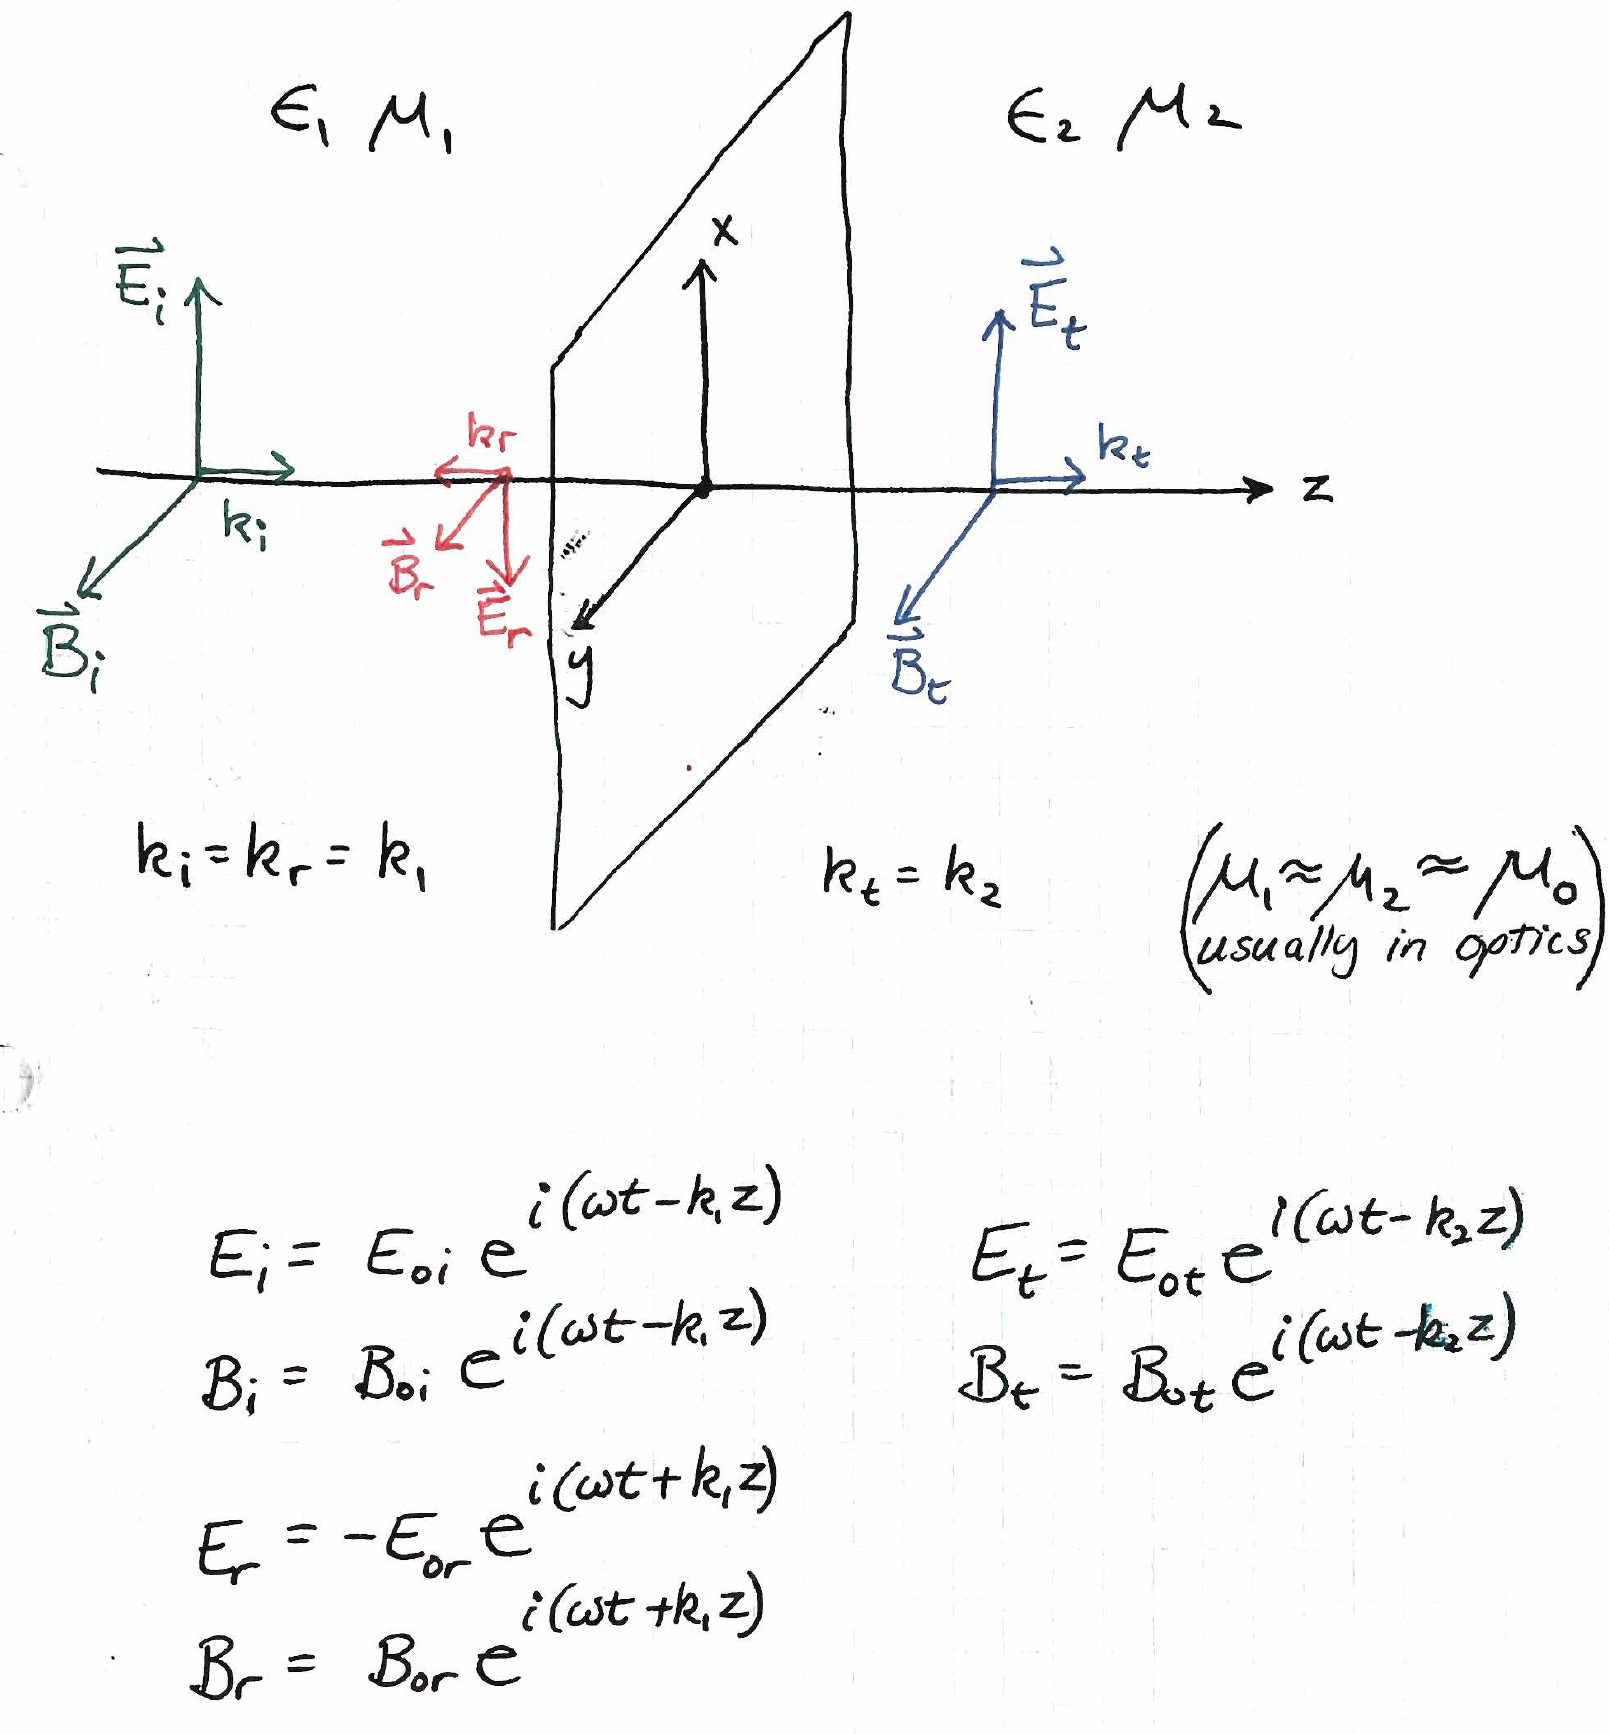
\includegraphics[width=\textwidth]{EandB.png}
\end{center}
where $k_n=\frac{\omega}{v_n}=\omega\sqrt{\mu_n\epsilon_n}$
\[E_r=E_i\left[ \frac{Z_1-Z_2}{Z_1+Z_2}  \right]\] and \[ E_t = E_i \left[ \frac{2Z_2}{Z_1+Z_2} \right]\]
With $Z_i=\mu_i v_i = \frac{\mu_i c}{n_i}$ gives:
\[E_r=E_i\left[ \frac{n_2-n_1}{n_1+n_2}  \right]\] and \[ E_t = E_i \left[ \frac{2n_1}{n_1+n_2} \right]\]
Reflection coefficient:
\[R=\left\vert\frac{E_r}{E_i}\right\vert^2=\left( \frac{n_2-n_1}{n_2+n_1} \right)^2\]
Transmission coefficient:
\[T=\frac{n_2\cos\theta_2}{n_1\cos\theta_1}\left( \frac{E_t}{E_i} \right)^2=\frac{4n_1n_2}{(n_1+n_2)^2}\]
Snell's Law:
\[n_1\sin\theta_1=n_2\sin\theta_2\]
Fresnel Formulae:
\begin{equation}
    \frac{E_{ot}}{E_{oi}}=1-\frac{E_{or}}{E_{oi}}=1-\left( -\frac{\cos\theta_1-\sqrt{\left(\frac{n_2}{n_1}\right)^2-\sin^2\theta_1}}{\cos\theta_1+\sqrt{\left(\frac{n_2}{n_1}\right)^2-\sin^2\theta_1}}  \right)
\end{equation}
\begin{equation}
    \frac{E_{ot}}{E_{oi}}=\frac{n_1}{n_2}\left[1+\frac{E_{or}}{E_{oi}}\right]=1+\left( \frac{\left(\frac{n_2}{n_1}\right)^2\cos\theta_1-\sqrt{\left(\frac{n_2}{n_1}\right)^2-\sin^2\theta_1}}{\left(\frac{n_2}{n_1}\right)^2\cos\theta_1+\sqrt{\left(\frac{n_2}{n_1}\right)^2-\sin^2\theta_1}}  \right)
\end{equation}
Where (11) is when E is perpendicular to the incidence plane, and (12) is when E is parallel to the incidence plane.\\
Brewster's Angle:
\[\theta_B=\tan^{-1}\left( \frac{n_2}{n_1}\right)\]
When the reflection and transmission are perpendicular to each other, and there will be 0 reflection. 
\\ Total internal reflection when $\theta_1>\theta_{crit}$, where
\[\sin\theta_{crit}=\frac{n_2}{n_1}\]
e-folding scale:
\[z_0=\frac{1}{k^2}\left( \frac{\sin^2\theta_1}{\sin^2\theta_{crit}} -1 \right)^{-1/2}\]


\end{document}